\usetikzlibrary{arrows.meta}
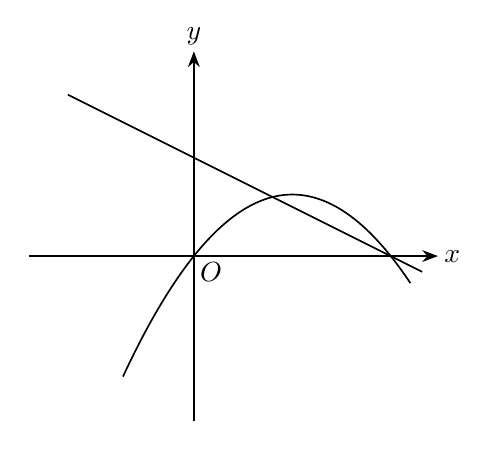
\begin{tikzpicture}[x=1cm,y=1cm,line width=.6pt,>=Stealth,font=\normalsize]
\draw[->] (-2.10,0)--(3.10,0) node[right,inner sep=0pt,xshift=2pt] {$x$};
\draw[->] (0,-2.10)--(0,2.60) node[above,inner sep=0pt,yshift=2pt] {$y$};
\node[below right,inner sep=0pt,xshift=2pt,yshift=-2pt] at (0,0) {$O$};
% consistent representative a=-1,b=2: parabola y=-x^2+2x roots 0,2
\draw[domain=-0.90:2.75,samples=120] plot (\x,{-0.5*\x*\x+1.25*\x});
% line y=-0.5x+1 shares origin relation and right intercept 2
\draw[domain=-1.60:2.90,samples=2] plot (\x,{-0.5*\x+1.25});
\end{tikzpicture}
